A Teoria Gravitacional proposta por Isaac Newton nos permite obter as equações de movimento para  dois corpos que se atraem mutuamente através da gravidade. Surge, no entanto, como decorrência dessa formalização uma complexa situação, na qual as ferramentas disponíveis tornam-se quase obsoletas, entraves caóticos provenientes da observação do chamado problema de três corpos. Diversos filósofos da natureza se debruçaram sobre a dinâmica envolvendo três corpos interagindo gravitacionalmente, buscando uma equação geral de movimento para as componentes do sistema. Cumpre ressaltar a importância particular de dois deles no que será abordado, avançando crucialmente a compreensão humana acerca dos referido problema: Leonhard Paul Euler, com sua primazia, e Joseph-Louis Lagrange, com o esclarecimento do que havia sido deixado em aberto pelo primeiro.
   
Esse avanço foi alcançado lançando mão de certas considerações. Na década de 60 do século XVIII, Euler modelou um sistema trinário unidimensional* e, com isso, indicou a existência de configurações estacionárias. Em suma, dados dois corpos, existem três pontos na reta que passa pelo centro de massa de ambos nos quais o posicionamento do terceiro corpo faz com que a distribuição relativa entre os três permaneça a mesma. Por conseguinte, seu aluno Lagrange, em 1772, dando prosseguimento as descobertas sobre equilíbrio no problema de três corpos, ao trabalhar em um sistema tridimensional, executando a maioria dos cálculos considerando apenas dois corpos e adicionando em seguida o terceiro, menos massivo*, obteve as posições de um quarto e um quinto ponto com a mesma propriedade estacionária dos anteriores. Dos cinco pontos citados, os três primeiros, descobertos por Euler, correspondem a pontos de equilibrio instável do sistema. Os demais, publicados por Lagrange, são estáveis. A todos eles dá-se o nome \textit{pontos de Lagrange}. A figura 1 retrata os pontos marcados como L1, L2, L3, L4 e L5.

\begin{figure}[!h]
\centering
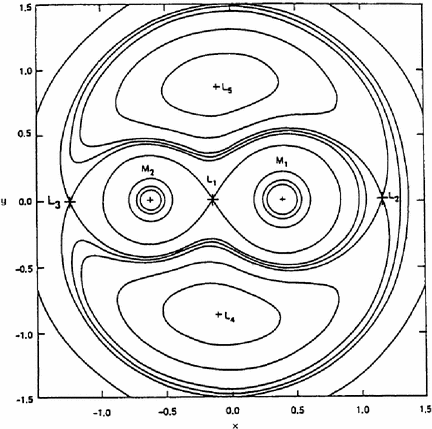
\includegraphics{PL.gif}
\caption{Curvas equipotenciais e pontos de Lagrange. Retirado de CITAR KEPLER DE SOUZA.}
\end{figure}
   
Em decorrência da estabilidade dos pontos, é natural o acúmulo de matéria nas regiões em volta de L4 e L5. Um exemplo claro disso, são os asteróides troianos de Júpiter: uma família de corpos celestes que se dispoem nos pontos de equilíbrio estável do sistema Sol-Júpiter. Os outros pontos, apesar de instáveis, são largamente utilizados por instrumentos de pesquisa espacial. O SOHO (Solar and Heliospheric Observatory -- Observatório Solar e Heliosférico)** se mantem numa órbita em volta do ponto L1 do sistema Sol-Terra, permitindo à sonda uma visão initerrupta do Sol, sem sofrer com eclipses causados pelo nosso planeta. Numa órbita em torno do ponto L2, há o WMAP (Wilkinson Microwave Anisotropy Probe -- Sonda de Anisotropia de Microondas Wilkinson)**, cuja localização lhe fornece uma visão clara do espaço profundo.

%   *: De motu rectilineo trium corporum se mutuo attrahentium (http://eulerarchive.maa.org//docs/originals/E327.pdf), Euler;
%      Essai sur le problème des trois corps (http://gallica.bnf.fr/ark:/12148/bpt6k229225j/f231.image.r=Oeuvres+de+Lagrange.langFR), Lagrange.

%   **: SOHO's Orbit (https://sohowww.nascom.nasa.gov/about/orbit.html);
%       WMAP Trajectory and Orbit (https://map.gsfc.nasa.gov/mission/observatory_orbit.html).

